%%
%% Author: jordan
%% 17/11/2018
%%

% Preamble
\documentclass[11pt]{article}

% Packages
\usepackage{amsmath, mathrsfs}
\usepackage{titling}
\usepackage{hyperref}
\usepackage[sorting=none]{biblatex}
\usepackage{graphicx}
\addbibresource{initialreport.bib}

\title{A new video analysis algorithm for the study of crowd dynamics}
\author{Jordan Osborn (jo357) Supervisor: Professor Pietro Cicuta (pc245)}
% Document
\begin{document}
\begin{titlingpage}
    \maketitle
\end{titlingpage}
\clearpage

\title{A new video analysis algorithm for the study of crowd dynamics}
\author{Supervisor: Professor Pietro Cicuta (pc245)}
\maketitle

\section{Introduction}
My part III project will be investigating the potential application of DDM (Differential Dynamic Microscopy) image processing techniques to videos of crowds in order to understand their dynamics.
DDM the method, first appeared in a paper written by R. Cerbino and V. Trappe in 2008.\cite{ddm0}
This project will be utilising a method derived from the initial one outlined in this paper.
In particular I will be making use of a fairly recently developed technique called multi-scale DDM.\cite{ddm1}
The aim of this project is to determine various dynamical properties of crowds such as how people move as a function of crowd density etc.
DDM analyses sequences of images and consists of a combination of difference and spatial fourier methods to discover information about the motion in the images.
A more in depth discussion will be carried out below.
These methods will first be developed on a standard PC to determine how best to apply them to the analysis of crowds.
The algorithms will then be optimised to run on an Nvidia Jetson TX2 development board (which would allow calculations to be more highly parallelised), the ultimate aim is to determine if we can use DDM to analyse crowd dynamics in real time.
By using this method we hope to be able to count people, density fluctuations, and discover other dynamical properties of crowds.
There are a few high quality crowd videos that are freely available in online databases.\cite{crowdMotionDB}
These will be used as the initial test data sets in the project.
The results of the algorithm will be compared with information gleaned from visual inspection of the videos and also as an extension possibly with the results of other video analysis techniques.
\\\\
Extensions to this project may include as mentioned previously implementations of other video analysis algorithms so that comparisons can be made with the results of the DDM method.
A camera may also be set up (utilising a raspberry pi) that would stream the contents of the video captured by the camera to the Nvidia Jetson TX2 over WiFi.
The algorithm could then be run on this streaming video and a test could be carried out to determine if the algorithm can be used to perform crowd analysis in realtime.
Another extension that might be possible is the development of a GUI that highlights certain features (based on the information found using DDM) in the crowd motion video in real time.
\\\\
If this project is successful in being able to measure crowd dynamics in real time then DDM may find an application in real time crowd safety/monitoring systems in crowded environments such as public transportation, stadiums, city centers etc.

%\section{Project Description}
%"This project will build on multi-DDM, a recently developed analysis technique from our group,
%and apply it for the first time to the study of collective motion in crowds.
%Videos from a data-bank will be used (a set of benchmark videos used in computer vision).
%Ideally the code will be compiled on CUDA and optimised to run in realtime on dedicated hardware (NVIDIA Jetson boards).
%The objective is to be able to count people, density fluctuations, flows, *without* segmenting the images or searching for features."

\section{Tools}
This project will make use of a wide variety of software and also hardware.
First off the algorithm will be written in a mixture of standard C++ and cuda (for the GPU relevant parts).
Python and PyCuda may also be used for less performance critical parts of the implementation.
Various libraries will likely be made use of including openCV, mathematical/graphing libraries and possibly Qt if a GUI is required at any point.
As for hardware the project will initially be utilising a standard computer to carry out the analysis.
But once there is a working implementation of the method it will be ported and optimisied to run on the Nvidia Jetson development board.
This will be done in order to increase the speed at which the algorithm runs, the benefit of running the algorithm on the Jetson
is that each frame may be stored on the GPU of the device and calculations can be carried out in parallel on that image.
Initially an online crowd motion database will be used as a test data set.\cite{crowdMotionDB}
This data set could be streamed to the Jetson to simulate a real time environment.
But as an extension a raspberry pi with an attached battery and camera could be set up to stream live videos of crowds over Wifi to the Jetson.
This could be used to test the potential application of DDM to real time analysis of crowd dynamics.
LaTeX will be used extensively to write up the results of this project.

\section{Background Physics and Mathematics}
DDM or Differential Dynamic Microscopy is a method that can be used to analyse an image sequence by taking a difference between two images (removes static features and retains only motion/differences between frames),
and then taking the 2D spatial fourier transform of this difference to obtain an image structure function.
From this function many properties of the motion can be determined.\cite{ddm1}
An outline of the mathematics is given below:
\\
\begin{equation}
    d(\textbf{r}, t_0, \tau) = I(\mathbf{r}, t_0 + \tau) - I(\mathbf{r}, t_0)
\end{equation}
The function $\textit{I}$ encodes the 2D projection of the scene along the optical axis of the camera (i.e the image intensity) as a function of position and of time.
This intensity could well be in colour (tuple of 3 intensities for red, green and blue) or could be in greyscale.
Colour information may provide extra information about motion but may also be an artifact produced by lighting effects.
Greyscale images would provide the necessary motion information and would not be vulnerable to the issues colour images may pose (more computational complexity, does a colour change really indicate motion etc.)

\begin{equation}
    \mathscr{F} (d(\textbf{r}, t_0, \tau) ) = \mathscr{F} (I(\mathbf{r}, t_0 + \tau) - I(\mathbf{r}, t_0)) = \mathscr{F}(I(\mathbf{r}, t_0 + \tau)) - \mathscr{F}(I(\mathbf{r}, t_0))
\end{equation}

The second equality results from the linearity of the fourier transform and reduces computational complexity as it allows you to cache fourier transforms at each time and then compute their difference.
This reduces the number of fourier transforms you need to compute, hence provides a computational optimisation.\cite{ddm2}
We now have

\begin{equation}
    d(\textbf{q}, t_0, \tau) ) = \mathscr{F}(I(\mathbf{r}, t_0 + \tau)) - \mathscr{F}(I(\mathbf{r}, t_0))
\end{equation}

Where $\textbf{q}$ is the 2d wave vector $(q_x, q_y)$.
Simplifications can be made if you can make some assumptions about the properties of the image, including isotropy and that motion is indifferent about the reference time (can average for all $t_0$).\cite{ddm1}
At this stage we will not make these assumptions as they may limit the applicability of the results found (motion is not likely to be isotropic as crowds tend to have an overall direction)
(reference time will also likely make a difference as the density of a crowd is likely to vary with time, over sufficiently small timescales this however may be a valid assumption).
We will use the more general result in the ddm algorithm and perhaps make adjustments if needed.

The wave-vectors can be used to derive a wavelength $(\lambda = \frac{2\pi}{|\textbf{q}|})$ which gives you the length scale probed by a particular mode.
Information about the system's dynamics can be obtained by looking at how the amplitudes of the fourier modes for each q changes with the time differences between frames $\tau$.\cite{ddm2}

A related method called multi-scale DDM (which is what this project will predominantly be using) picks up temporal and spatial scales of synchronisation separately (normal DDM only picks up a combination).
In multi-scale DDM you perform a normal DDM over a whole series of different tilings of the image.\cite{ddm1}
These tilings are chosen so that windows vary from a full scale image down to the smallest tile size (determines the minimum wave-vector that can be compared across tiles) (usually log spaced)\cite{ddm1}
To reduce the number of tiles that need to be computed you can select only the tiles showing the most activity, an equation that can determine if a tile exceeds a threshold activity is
\begin{equation}
    \Sigma_{\textbf{r} \in tile} \sigma(\textbf{r}) = \Sigma_{\textbf{r} \in tile} \sqrt{\frac{\Sigma_{[t_0, t_0 + \tau]} (I(\mathbf{r}, t) - <I(\mathbf{r}, t)>)^2}{N - 1}} > \sigma_{threshold}
\end{equation}

Which sums all of the standard deviations (computed over the time period $\tau$) of the intensities at each position in the tile and then checks if this sum is greater than some threshold standard deviation.
If it is a valid inequality then that tile is said to be "active" otherwise it is "inactive".\cite{ddm2}
This is a very rudimentary activity classifying function.
There are other ways that a tile's activity can be classified which may need to be investigated.

In the cross comparisons between the tiles of different sizes the scale of the collective motion should emerge.\cite{ddm1}
Other properties of the motion should emerge by studying how tau varies as a function of the wave-vector amplitude.\cite{ddm1}

The information provided by the multi-scale ddm method can be used to compute a variety of spatial and temporal properties of both collective and individual motion.\cite{ddm1}\cite{ddm2}

Benefits of this method include:
\begin {enumerate}
 \item does not require the segmentation of images (can study small objects).
 \item no need to track features across frames (denser systems can be studied).
 \item it requires no user defined parameters (can run autonomously).
\end{enumerate}\cite{ddm1}

\begin{figure}
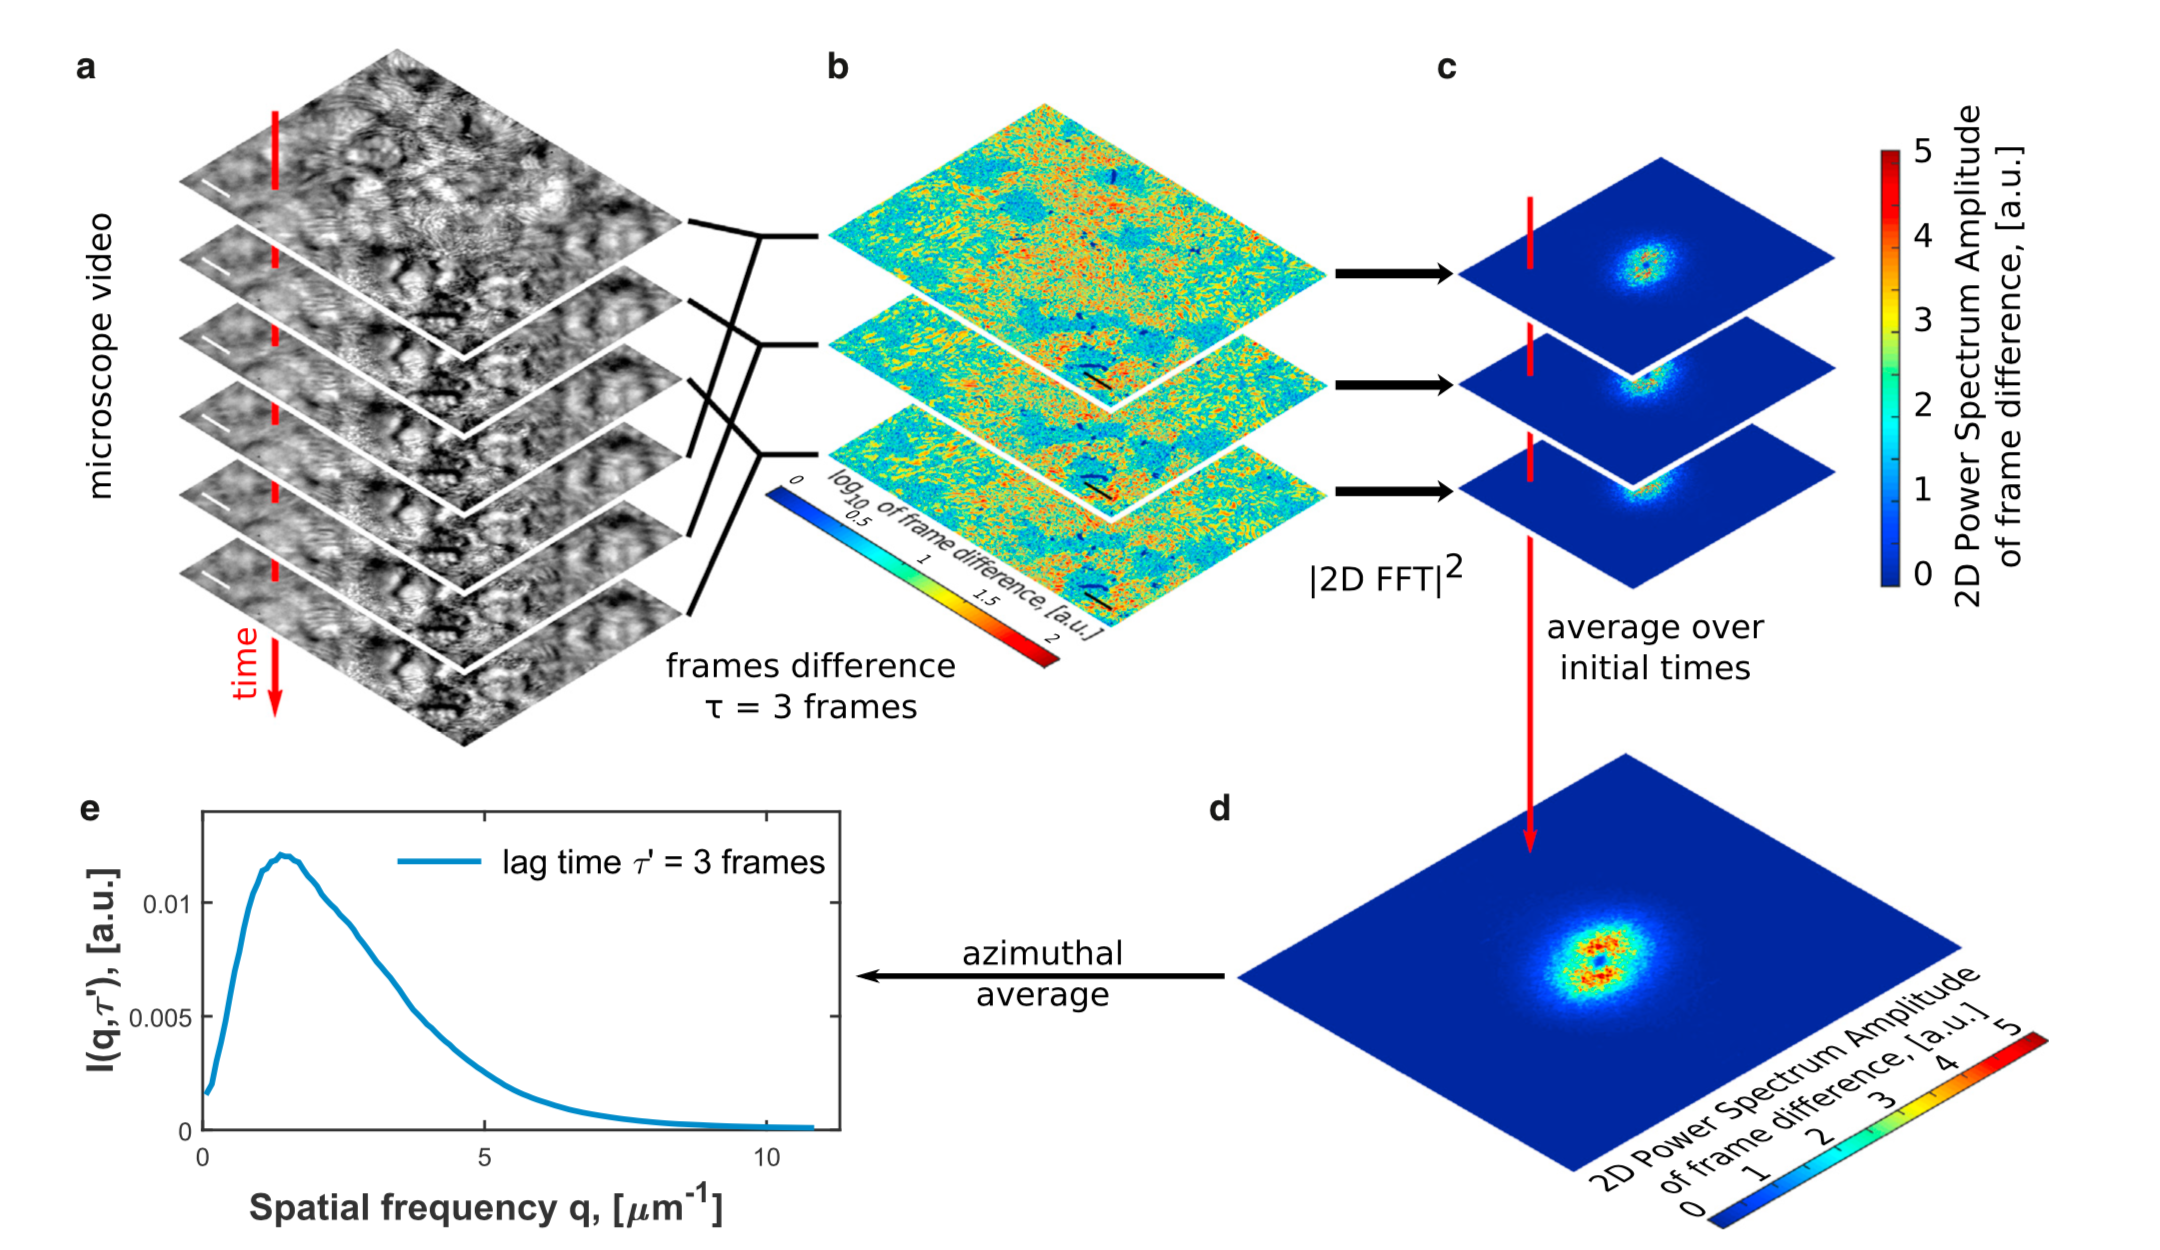
\includegraphics[width=15cm, height=6cm]{ddmpic.png}
\caption{Provides an overview of the ddm method as applied to the analysis of collective dynamics in ciliated cells.
In (a) we see the video frames in an ordered sequence.
In (b) the difference between frames separated by ($\tau=3 frames$) is shown.
The modulus squared of the 2D spatial fourier transform is displayed in (c).
(d) and (e) are less relevant to our use-case as we will not be assuming a stationary, ergodic and isotropic sample.
So we will not be averaging over initial times or averaging azimuthally.\cite{ddm2}}
\end{figure}

\section{Project Plan}
The project will effectively be split in to two stages, the implementation phase and the analysis phase.

\subsection{Implementation}
Over the Christmas vacation I plan to study from a book I discovered that goes in to depth about cuda, openCV and image analysis in general.\cite{cuda_book}
I am going to read this so that I will be ready to start implementing the algorithms come January.
Once I have finished this preliminary study, I will start implementing the DDM algorithm on a standard pc using C++.
This should provide some initial data and insights in to how the DDM method should be implemented in cuda on the Jetson development board.
And where optimisations might need to be carried out in order to arrive at a method that can be used in real time.
I will then start to alter the code so that it will run on and utilise the GPU of the Jetson development board.
I will also perform further optimisations at this stage so that the ultimate aim of real time crowd analysis might be achieved.
At each step videos from \url{http://mmlab.ie.cuhk.edu.hk/projects/collectiveness/dataset.htm}\cite{crowdMotionDB} and other online sources will be used to test the implementation.
\\
Once the main implementation has been completed further enhancements may be made (time permitting) including:
\begin{enumerate}
\item Further optimisations to the speed of the algorithm.
\item Using real live crowd video from a camera attached to a raspberry pi (streamed via Wifi to the Jetson) as input.
\item Comparisons to other motion analysis techniques.
\item GUI that highlights/graphs features in the video streams in real time (person count, flow direction, density charts etc.)
\end{enumerate}

\subsection{Analysis and Write Up}
Analysis will be carried out alongside and also after completion of the implementation phase.
The aim of the analysis is to determine individual and collective properties of the motion of the crowd.
These might include a person count, density fluctuations and flows in the crowd.
These will be determined by analysing the output of the DDM algorithm.
Multi-scale DDM provides both spatial and temporal information about the motion in a video.
The information provided by the algorithm will be analysed to determine the features mentioned above.
Graphs over time of these features will be made and included in a report with discussions about what they mean.
The data's claims will be compared with those inferred from visual inspection of the videos and also (time permitting) the results from other motion analysis algorithms.
A final report will be produced containing the implementation details and the analysis of the conclusions drawn from the results provided by the algorithm.
Pitfalls, benefits, improvements and potential applications will be discussed in the report.
And finally a discussion about whether real time crowd analysis was achieved (if not whether it would be possible and what would be required if so) and if shortcuts were needed to achieve this (lower precision etc.).

\section{Conclusion}
The project will be an investigation about how a method originally developed in the field of microscopy might be utilised in other fields.
It will investigate the potential application of this method to the analysis of crowd dynamics.
An exploration in to what information can be extracted from crowd motion videos using multi-scale DDM will be a significant part of this project.
The DDM method will be compared to other existing motion analysis techniques and a discussion about whether it provides any benefits/drawbacks to existing techniques will be had.
The ultimate aim of the project is to determine if real time analysis of crowd dynamics is possible using the DDM method on commercial hardware.

\printbibliography

\end{document}
